% IEEEAerospace2012.cls requires the following packages: times, rawfonts, oldfont, geometry
\documentclass[twocolumn,letterpaper]{IEEEAerospaceCLS}  % only supports two-column, letterpaper format

% The next line gives some packages you may find useful for your paper--these are not required though.
%\usepackage[]{graphicx,float,latexsym,amssymb,amsfonts,amsmath,amstext,times,psfig}
% NOTE: The .cls file is now compatible with amsmath!!!

\usepackage[]{graphicx}    % We use this package in this document
\newcommand{\ignore}[1]{}  % {} empty inside = %% comment

\begin{document}
\title{An Example of the 2020 IEEE Aerospace Conference Paper Format Using a \LaTeX~Environment}

\author{%
Erica Deionno\\ 
The Aerospace Corporation\\
2310 E. El Segundo Blvd.\\
El Segundo, CA 90245\\
erica.deionno@aero.org
\and 
Jane Smith\\
Department of ECE\\
University of Nowhere\\
Nowhere, ZS 99999\\
jane.smith@nowhere.edu
%%%% IMPORTANT: Use the correct copyright information--IEEE, Crown, or U.S. government. %%%%%
\thanks{\footnotesize 978-1-7281-2734-7/20/$\$31.00$ \copyright2020 IEEE}              % This creates the copyright info that is the correct 2020 data.
%\thanks{{U.S. Government work not protected by U.S. copyright}}         % Use this copyright notice only if you are employed by the U.S. Government.
%\thanks{{978-1-7281-2734-7/20/$\$31.00$ \copyright2020 Crown}}          % Use this copyright notice only if you are employed by a crown government (e.g., Canada, UK, Australia).
%\thanks{{978-1-7281-2734-7/20/$\$31.00$ \copyright2020 European Union}}    % Use this copyright notice is you are employed by the European Union.
}



\maketitle

\thispagestyle{plain}
\pagestyle{plain}


\begin{abstract}
This paper serves as an example for the use of the \LaTeX~class file for the 2020 Aerospace Conference. The \LaTeX~class file for the 2020 conference has been modified from that of prior year conferences in order to fix minor bugs and to conform to new formatting requirements. Within the class file there are some customized commands that are illustrated in this paper. They are: tableofcontents, acknowledgments, thebiography. There are also comments sprinkled throughout the~.tex file to illustrate the usage of the class file. If you have difficulties or errors using this class file, please contact me at the e-mail address in the author's information slot. Some of the content below is filler designed to show you how a properly formatted paper should look. Read the official ``Author's Instructions for the 2020 IEEE Aerospace Conference'' to find the full description of the paper formatting requirements.
\end{abstract}


\tableofcontents

%%%%%%%%%%%%%%%%%%%%%%%%%%%%%%%%%%%%%%
\section{Introduction}
%%%%%%%%%%%%%%%%%%%%%%%%%%%%%%%%%%%%%%
The annual IEEE Aerospace Conference is a venue for engineers and scientists to present their work to one another. Please submit a paper only if you or a coauthor are committed to attend and present it personally.

An IEEE Aerospace Conference paper is comprised of standard parts described in Section 2 of this paper. Section 3 briefly describes the manuscript style and Section 4 the submission deadlines and procedures. Section 5 discusses presentation of papers at the conference. The Best Paper Awards and paper publication are described in Section 6. Section 7 provides a summary.

Proper formatting of your paper as specified in this document contributes to the successful production of these documents. All papers are also published in PDF format on the {\it IEEE Xplore} web-based system, shortly after the conference concludes.

A double-column format is required, although figures, tables, and equations may be full-page width. Specifications are listed for typeface, type size, headings, column separation, margins, and other style parameters.

Where this document is silent on a formatting question, it is because it is not important or is the writer's option. When in doubt make a choice that makes your document most readable. English is the official language of the conference, and the official page size is 8.5 x 11 inches--do not use A4 paper size.



%%%%%%%%%%%%%%%%%%%%%%%%%%%%%%%%%%%%%%%%%%%
\section{Paper Organization}
%%%%%%%%%%%%%%%%%%%%%%%%%%%%%%%%%%%%%%%%%%%
IEEE papers consist of a minimum of nine parts.

\subsection{Title}
The title should indicate the subject of the paper as briefly as possible. The maximum length, including spaces, is 100 characters.

\subsection{Author(s)}
Names of all authors, their affiliations, postal addresses, and e-mail addresses should follow the title, centered on the full width of the page. Do not include titles or degrees except for military rank. Multiple authors may be listed two or three across and as deep as needed. Large numbers of authors should be grouped by address.

\subsection{Abstract}
An abstract of 250 to 500 words should concisely describe the work being reported, its methodology, principal results and significance.

\subsection{Table of Contents}
Major headings and their page numbers are listed in the Table of Contents.

\subsection{Introduction}
The introduction provides background information, such as previous work, and describes how the paper is organized.

\subsection{Body}
The body describes the work in detail and discusses its application. The body should be organized into logical sections with headings and subheadings and be illustrated with figures and tables. Subsidiary information can be relegated to footnotes.

\subsection{Conclusions}
Conclusions should clearly state principal results of the work, its significance, limitations, advantages, and applications. Recommendations for further work are also encouraged.

\subsection{References}
List and number all bibliographical references at the end of the paper.

\subsection{Biography}
Provide a short biography for each author, which can include title, fields of expertise, work experience, education, and relevant personal information. Also include a 1.25 inch wide x 1.5 inch high headshot (at 300 dpi) of each author.

\subsection{Additions}
Add appendices and acknowledgments, if appropriate.



%%%%%%%%%%%%%%%%%%%%%%%%%%%%%%%%%%%%%%%%%%%%%
\section{Manuscript Style}
%%%%%%%%%%%%%%%%%%%%%%%%%%%%%%%%%%%%%%%%%%%%%

\subsection{Paper Length}
The paper may be 6 to 20 pages in length.

\subsection{Copyright Notice}
A copyright notice must be placed as a footnote on the first page of the paper. Do not number this footnote. Choose an appropriate alternative from the list of four below:
\begin{itemize}
  \item [(1)] For papers in which all authors are employed by the US government, the copyright notice is: \textbf {U.S. Government work not protected by U.S. copyright} \\
  \item [(2)] For papers in which all authors are employees of a Crown Government (UK, Canada, Australia), the copyright notice is: \\{\bf 978-1-7281-2734-7/20/\$31.00 \copyright2020 Crown}\\
  \item [(3)] For papers in which all authors are employed by the European Union, the copyright notice is: \\{\bf 978-1-7281-2734-7/20/\$31.00 \copyright2020 European Union}\\
  \item [(4)]  For all other papers the copyright notice is: \\{\bf  978-1-7281-2734-7/20/\$31.00 \copyright2020 IEEE}
\end{itemize}


\subsection{Paper, Margins, and Spacing}
Format your electronic submission to 8.5 x 11 inch page size in double-column format with 0.75 inch margins on each side, top and bottom. There should be 0.25 inch between columns, which are justified both right and left.

Lines of text should be single-spaced, except for double spacing before headings and space-and-a-half after.

\subsection{Headers and Footers}
No headers are permitted. Utilize footers only for page numbers, which are centered at the bottom of each page.

\subsection{Headings}
\subsubsection{Major Headings}
Centered in the column with a double space before and space-and-a-half after.
\subsubsection{Subheadings}
Italicized and placed flush on the left-hand margin on a separate line. Use a double space before and space-and-a-half after.
\subsubsection{Subsubheadings}
Italicized, followed by an em dash and run in at the beginning of the paragraph. This paragraph has a correctly formatted subsubheading.

\subsection{Other Elements}
\subsubsection{Equations}
Equations should be centered in the column. When numbering an equation, enclose the number in parentheses placed flush with the right-hand margin of the column, as shown in the sample equations that follow.
\begin{equation}
{\bf F}=m{\bf a}
\end{equation}
\begin{equation}
e=mc^2
\end{equation}

Mathematical derivations and proofs should be developed in appendices.

\subsubsection{Figures}
Place figures as close to the text reference as possible. Center figure titles directly below the figure, as shown in Figure 1.

Figures should be sized for easy reading. No lettering in a figure should be smaller than 10 points. Scan photographs at a 300-dpi resolution and embed them in the paper. High-resolution images should be reduced to 300 dpi at the size they will be printed.

\begin{figure*}
\centering
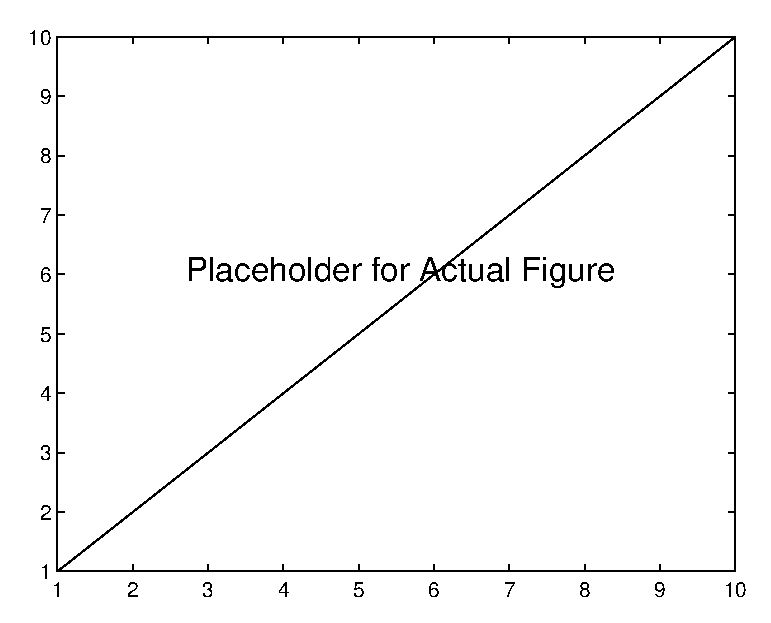
\includegraphics[width=4in]{Placeholder.eps}
\caption{\bf{Here is an example of a figure that spans both columns.}}
\label{FlowChart}
\end{figure*}

\subsubsection{Tables}
Place tables as close to the text reference as possible. Use the full width of the page for legibility, if required. Center table titles directly {\bf above} the table.

\subsubsection{Footnotes}
All footnotes\footnote{\bf This is an example of a footnote.} following the IEEE copyright notice are numbered consecutively. 

%%%%%%%%%%%%%%%%%%%%%%%%%%%%%%%%%%%%%%%%%%%%%%%%%%%%%
\section{Paper Submission}
Submission due dates and deadlines are given in Table \ref{DueDates}.

\begin{table}
\renewcommand{\arraystretch}{1.3}
\caption{\bf Summary of Due Dates}
\label{DueDates}
\centering
\begin{tabular}{|c|c|}
\hline
\bfseries Event & \bfseries Due Date \\
\hline\hline
Abstracts Due               & July 1, 2019 \\
Review Paper Deadline & October 18, 2019 \\
Final Revised Paper Deadline          & January 8, 2020\\
IEEE Copyright Form Due     & January 8, 2020\\
\hline
\end{tabular}
\end{table}

\subsection{Abstract}
An abstract of 250 to 500 words describing the planned content of the paper must be submitted electronically at the conference website.

\subsection{Review Paper}
The paper submitted for review must be a complete, fully formatted, and proofread manuscript, ready for publication. NO paper submitted for review after the deadline will be reviewed or admitted to the conference.

\subsection{Final Paper}
Following receipt of review comments, make appropriate revisions to the paper and submit a final version for publication.

\subsection{IEEE copyright Form}
An IEEE Copyright Release Form for each paper, signed by the author or author's employer, is due with the final paper. 

Copyright forms are available at the conference website and can be submitted electronically at the IEEE site linked for this purpose or by mail to the address provided on the website.

\subsection{ITAR Compliance}
International Traffic in Arms Regulation (ITAR) controls the export and import of defense articles and defense services as detailed in the U.S. Munitions List \cite{ITAR}.

Authors who are U.S. nationals (including green card holders), work for a U.S.-based organization regardless of where they are physically located, or work at a U.S. location of a non-U.S.-based organization, must ensure that ITAR compliance has been obtained for any and all papers submitted to IEEE for publication.

\subsection{Organizational Approval}
Authors are expected to obtain any needed clearances for their work to be freely published by the IEEE. Submission of your paper implies that it has received the proper clearances from your company, affiliation, or organization.

\subsection{Submission to the \underline{www.aeroconf.org} website}
Before Submitting your abstract or paper:
\begin{itemize}
  \item [1)] Scan your document with a current anti-virus product. (If a virus is detected, your file willl be deleted) \\
  \item [2)] Remove passwords or other protection from your file that would prevent it from being opened. \\
  \item [3)] Submit a PDF version of your abstract of paper via the website.
\end{itemize}

%%%%%%%%%%%%%%%%%%%%%%%%%%%%%%%%%%%%%%%%%%%%%%%%%%%%%
\section{Presentation at the Conference}
%%%%%%%%%%%%%%%%%%%%%%%%%%%%%%%%%%%%%%%%%%%%%%%%%%%%%
Prepare a presentation to be delivered at the conference, using Microsoft PowerPoint or similar software, that summarizes the major concepts of your paper.

\subsection{Allotted Time}
Time allotted for presentations is 18 minutes, with an additional 5 minutes for questions. The time limit will be strictly enforced.

\subsection{Projection}
A projector and screen will be set up in each meeting room. Bring your slide set on a laptop to plug in to the projector. Also bring a copy of your presentation on a USB drive, in case your session chair chooses to consolidate all the presentations on a single laptop before the session starts.

\subsection{Presentation}
Tips on giving the presentation will be sent to registered authors in advance of the conference.


\subsection{Special Displays}
Displays of hardware or software an author believes to be of wide interest to conference attendees may be set up with permission of the Technical Program Committee and by special arrangement with the Conference Manager.

%%%%%%%%%%%%%%%%%%%%%%%%%%%%%%%%%%%%%%%%%%%%%%%%%%%%%
\section{Best Paper Award and Publication}
%%%%%%%%%%%%%%%%%%%%%%%%%%%%%%%%%%%%%%%%%%%%%%%%%%%%%
\subsection{Best Paper Award}
Awards for Best Paper Award in each track and the overall conference are given each year for excellence in technical innovation and exposition in the written paper. The selection is conducted prior to the conference and the award is presented at the conference.

\subsection{Publication}
Papers presented at the IEEE Aerospace Conference are published in two forms:
\begin{itemize}
  \item [1)] On an online database accessible by registrants \\
  \item [2)] In the official Conference Proceedings on the web-based {\it{IEEE Xplore}} System following the conference
\end{itemize}



\begin{figure}\label{OneColumn}
\centering
\includegraphics[width=3.25in]{placeholder.eps}\\
\caption{\textbf{ A single column figure.}}
\end{figure}


%%%%%%%%%%%%%%%%%%%%%%%%%%%%%%%%%%%%%%%%%%%%%%%%%%%%%
\section{Summary}
%%%%%%%%%%%%%%%%%%%%%%%%%%%%%%%%%%%%%%%%%%%%%%%%%%%%%
This Author's Instructions document serves as a template for papers prepared for the 2020 IEEE Aerospace Conference. All paper submissions are accomplished online, through the IEEE Aerospace Conference website at \underline {www.aeroconf.org} \cite{AeroConf}.





%%%%%%%%%%%%%%%%%%%%%%%%%%%%%%%%%%%%%%%%%%%%%%%%%%%%%%%%%%%%%%%%%%%%%%%%%%%%%%%%%%%%%%%%%%%%%%%%%
\appendices{}              % note there is no {} to put a title. Each appendix has its own title
%%%%%%%%%%%%%%%%%%%%%%%%%%%%%%%%%%%%%%%%%%%%%%%%%%%%%%%%%%%%%%%%%%%%%%%%%%%%%%%%%%%%%%%%%%%%%%%%%
% For a single appendix, use the \appendix{} keyword and do not use the \section command.

\section{More Information}        % first appendix
%%%%%%%%%%%%%%%%%%%%%%%%%%
This is the first appendix. 

\subsection{Comments}
If you have only one appendix, use the ``appendix'' keyword.

\subsection{More Comments}
Use section and subsection keywords as usual.

\section{Yet More Information}    % second appendix
%%%%%%%%%%%%%%%%%%%%%%%%%%%%%%
This is the second appendix.



%%%%%%%%%%%%%%%%%%%%%%%%%%%%%%%%%%%%%%%%%%%%%%%%%%%%%%%%%%%%%%%%%%%%%%%%%%%%%%%%%%%%%%%%%%%%%%%%%%%%%%
\acknowledgments
Project sponsors may be acknowledged in this section. 



%%%%%%%%%%%%%%%%%%%%%%%%%%%%%%%%%%%%%%%%%%%%%%%%%%%%%%%%%%%%%%%%%%%%%%%%%%%%%%%%%%%%%%%%%%%%%%%%%%%%%%
\bibliographystyle{IEEEtran}
%\bibliography{IEEEabr,MyBibFile}
\begin{thebibliography}{1}

\bibitem{ITAR}
U.S. Munitions List, Sections 38 and 47(7) of the Arms Export Control Act (22 U.S.C 2778 and 2794(7).

\bibitem{AeroConf}
Aerospace Conference Web site: \underline{www.aeroconf.org}.

\end{thebibliography}


%%%%%%%%%%%%%%%%%%%%%%%%%%%%%%%%%%%%%%%%%%%%%%%%%%%%%%%%%%%%%%%%%%%%%%%%%%%%%%%%%%%%%%%%%%%%%%%%%%%%%%
\thebiography
%% This biostyle allows you to insert your photo size 1in X 1.25in
\begin{biographywithpic}
{Erica DeIonno}{DeIonno.eps}
received her B.S./M.S. and Ph.D. degrees in chemistry from UCLA. She currently works in the Innovation Office at The Aerospace Corporation and is responsible for selected internal research programs, university collaborations, and technical communications. Before her current role, she spent 10 years in the Physical Sciences Laboratories. Her work included radiation testing and modeling of emerging resistive RAM technologies and space degradation modeling and lifetime predictions of solar cells and arrays.
\end{biographywithpic} 

\begin{biographywithpic}
{Jane Smith}{blankpic.eps}
received her B.S. degree in Electrical Engineering in 1985 and a Ph.D. in Aerospacel Engineering from the Massachusettes Institute of Technology in 1990. She is currently a professor of Aerospace Engineering at the University of Nowhere. Her interests include secure communications and space exploration.

\end{biographywithpic}




\end{document}
